\chapter{Membangun Model Prediksi}

Untuk pratikum saati ini menggunakan buku \textit{Python Artificial Intelligence Projects for Beginners}\cite{eckroth2018python}. Dengan praktek menggunakan python 3 dan editor anaconda dan library python scikit-learn.
Dataset ada di https://github.com/PacktPublishing/Python-Artificial-Intelligence-Projects-for-Beginners .
Tujuan pembelajaran pada pertemuan pertama antara lain:
\begin{enumerate}
\item
Mengerti implementasi klasifikasi
\item
Memahami data set, training dan testing data
\item
Memahami Decission tree.
\item
Memahami information gain dan entropi.
\end{enumerate}
Tugas dengan cara dikumpulkan dengan pull request ke github dengan menggunakan latex pada repo yang dibuat oleh asisten riset. Kode program menggunakan input listing ditaruh di folder src ekstensi .py dan dipanggil ke latex dengan input listings. Tulisan dan kode tidak boleh plagiat, menggunakan bahasa indonesia yang sesuai dengan gaya bahasa buku teks.

\section{Teori}\\
Nur Ikhsani Suwandy Futri\\
1194029\\
Praktek teori penunjang yang dikerjakan(nilai 5 per nomor, untuk hari pertama) :
\begin{enumerate}
\item
Jelaskan apa itu binary classification dilengkapi ilustrasi gambar sendiri\\

\begin{figure}[!htbp]
		\centering
		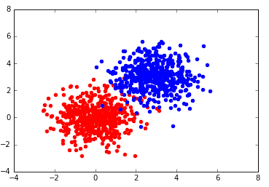
\includegraphics[scale=0.4]{figures/chapter2/binary.png}
	\end{figure}
	 \newpage

binary classification adalah tugas mengklasifikasikan suatu elemen-elemen dari himpunana yang diberikan ke dalam dua kelompok, dengan berdasarkan aturan klasifikasi. konteks yang dapat membutuhkan suatu keputusan pada suatu item yang memiliki sifat kualitatif atau tidak, adapun beberapa klasifikasi biner khas yaitu :\\
-Tes medis yang digunakan untuk melakukan keputusan pasien mempunyai penyakit tertentu atau tidak properti klasifikasi yaitu keberadaan penyakit.\\
-Mode uji yaitu lulus atau gagalnya suatu kontrol pabrik yang dapat memutuskan apakah suatu spesifikasi telah terpenuhi.\\
-Pengambilan informasi yaitu melakukan pemutusan suatu halaman atau artikel harus dalam hasil pencarian atau tidak properti klasifikasi yaitu relevan artikel.
\item
Jelaskan apa itu supervised learning dan unsupervised learning dan clustering dengan ilustrasi gambar sendiri.
\begin{figure}[!htbp]
		\centering
		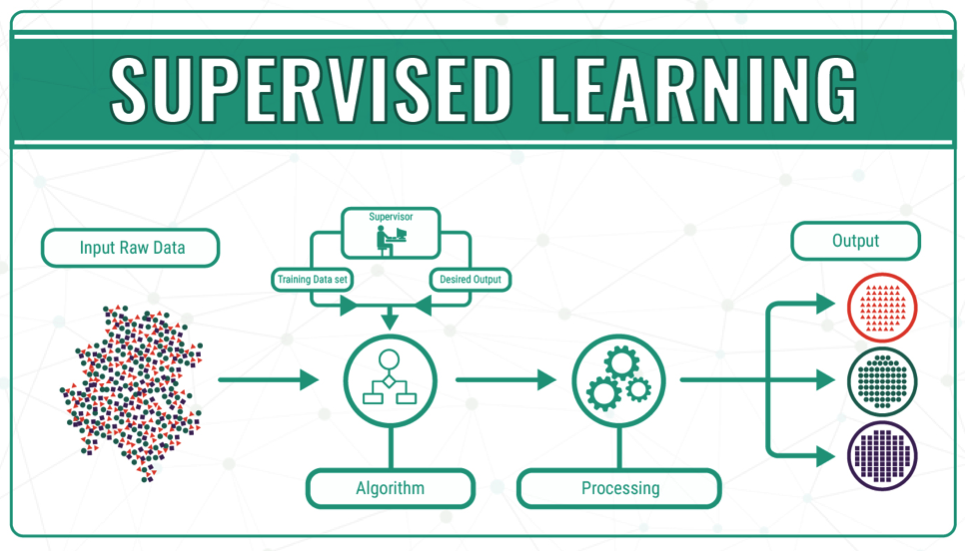
\includegraphics[scale=0.4]{figures/chapter2/supervised.png}
		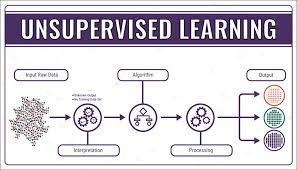
\includegraphics[scale=0.4]{figures/chapter2/unsupervised.jpeg}
		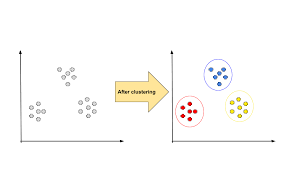
\includegraphics[scale=0.4]{figures/chapter2/clustering.png}
    \end{figure}
    \newpage
1. Supervised adalah suatu pendekatan machine learning yang dapat ditentukan dengan berdasarkan penggunaan dataset berlabel.\\
2. Unsepervised learning adalah suatu metode pembelajaran dengan menggunakan algoritma machine learning yang dapat digunakan untuk menganalisis serta mengelompokkan kumpulan data yang tidak berlabel.\\
3. Clustering adalah suatu metode penganalisaan data yang sering dimasukkan pada salah satu metode data maining yang mempunyai tujuan untuk mengelompokkan data dengan karakteristik yang sama pada satu wilayah yang sama dengan data.
\item
Jelaskan apa itu evaluasi dan akurasi dari buku dan disertai ilustrasi contoh dengan gambar sendiri.\\
\begin{figure}[!htbp]
		\centering
		
\includegraphics[scale=0.4]{figures/chapter2/evaluasi.png}
		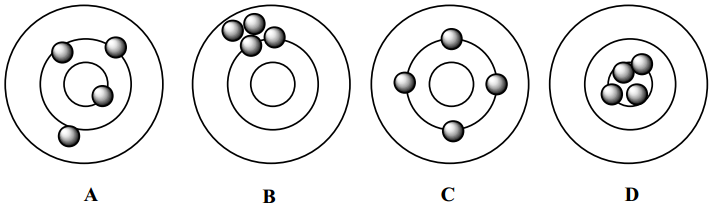
\includegraphics[scale=0.4]{figures/chapter2/akurasi.png}
    \end{figure}
    \newpage
Evaluasi adalah suatu kegiatan yang terencana agar dapat mengukur menilai dan keberhasilan suatu program, evaluasi juga merupakan suatu cara yang terbaik untuk menguji efektivitas dan produktifitas.\\
Akurasi adalah suatu ukuran kedekatan dari hasil pengukuran dengan niali yang sebenarnya atau nilai target.
\item
Jelaskan bagaimana cara membuat dan membaca confusion matrix, buat confusion matrix buatan sendiri.
\begin{figure}[!htbp]
		\centering
		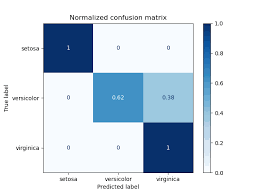
\includegraphics[scale=0.4]{figures/chapter2/confusion.png}
    \end{figure}
    \newpage
\item
Jelaskan bagaimana K-fold cross validation bekerja dengan gambar ilustrasi contoh buatan sendiri.
\begin{figure}[!htbp]
		\centering
		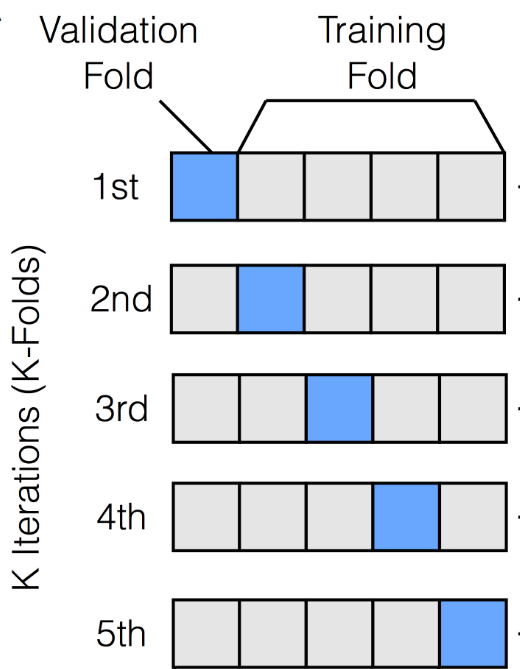
\includegraphics[scale=0.4]{figures/chapter2/k-fold.png}
    \end{figure}
    \newpage
K-fold cross validation adalah suatu metode yang digunakan untuk mendapatkan kinerja classifier, metode ini digunakan dengan jumlah data yang terbatas.
cara kerja K-fold cross validation yaitu \\
- total intance dibagi menjadi N bagian.\\
- fold-1 ketika bagian 1 manjadi data uji dan yang lainnya menjadi data pelatihan. sehingga dapat dihitung keakuratan berdasarkan porsi data. perhitungan akuasi menggunakan persamaan berikut Akurasi = sigma data uji benar klasifikasi sigma total data uji x 100.\\
- fold 2 pada bagian ke-2 menjadi data uji dan yang lainnya menjadi data pelatihan. sehingga hitung keakuratan berdasarkan porsi data 4 hingga seterusnya mencapai fold ke- K. pada hitungan rara-rata akursi dari K buah akurasi pada bagian atas. rata-rata akurasi ini menjadi akurasi final.
\item
Jelaskan apa itu decision tree dengan gambar ilustrasi contoh buatan sendiri.
\begin{figure}[!htbp]
		\centering
		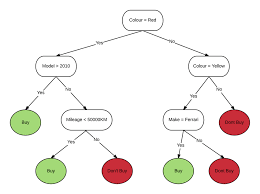
\includegraphics[scale=0.4]{figures/chapter2/decision.png}
    \end{figure}
    \newpage
Decision tree adalah alat pendukung dengan struktur seperti pohon yang memodelkan kemungkinan hasil, biaya sumber daya, utilitas, dan kemungkinan konsekuensi. Decision tree menyediakan cara untuk menyajikan algoritma dengan pernyataan kontrol bersyarat. Mereka termasuk cabang yang mewakili langkah-langkah pengambilan keputusan yang dapat mengarah pada hasil yang menguntungkan.
\item
Jelaskan apa itu information gain dan entropi dengan gambar ilustrasi buatan sendiri.
\begin{figure}[!htbp]
		\centering
		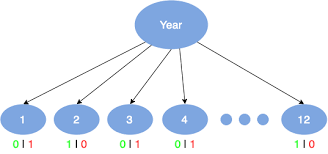
\includegraphics[scale=0.4]{figures/chapter2/informasigain.png}
		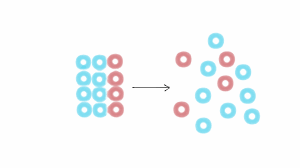
\includegraphics[scale=0.4]{figures/chapter2/entropi.png}
    \end{figure}
    \newpage
Informasi gain adalah  teknik seleksi fitur yang memakai metode  scoring untuk nominal ataupun pembobotan atribut kontinu yang didiskretkan menggunakan maksimal entropy. Suatu entropy  digunakan untuk mendefinisikan nilai Information Gain. Entropy menggambarkan banyaknya informasi  yang  dibutuhkan  untuk mengkodekan  suatu  kelas.\\
Entropi adalah salah satu besaran termodinamika yang mengukur energi dalam sistem per satuan temperatur yang tak dapat digunakan untuk melakukan usaha.
\end{enumerate}

\section{scikit-learn}
Dataset ambil di https://github.com/PacktPublishing/Python-Artificial-Intelligence-Projects-for-Beginners folder Chapter01.
Tugas anda adalah, dataset ganti menggunakan \textbf{student-mat.csv} dan mengganti semua nama variabel dari kode di bawah ini dengan nama-nama makanan (NPM mod 3=0), kota (NPM mod 3=1), buah (NPM mod 3=2), . Jalankan satu per satu kode tersebut di spyder dengan menggunakan textit{Run current cell}. Kemudian Jelaskan dengan menggunakan bahasa yang mudah dimengerti dan bebas plagiat dan wajib skrinsut dari komputer sendiri masing masing nomor di bawah ini(nilai 5 masing masing pada hari kedua).

\begin{enumerate}

\item
\begin{verbatim}
	# load dataset (student mat pakenya)
	import pandas as pd
	d = pd.read_csv('student-mat.csv', sep=';')
	len(d)//
	saya Nur Ikhsani Suwandy Futri 1194029 mod 3 = 2 jadi menggunakan buah.//
\end{verbatim}
\begin{figure}[!htbp]
		\centering
		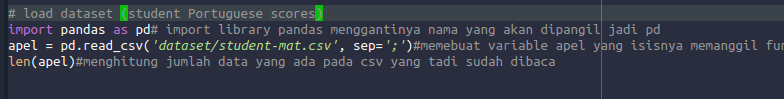
\includegraphics[scale=0.4]{figures/chapter2/chapter1.1.PNG}
		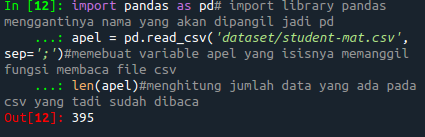
\includegraphics[scale=0.5]{figures/chapter2/hasilchapter1.1.PNG}
	\end{figure}
\newpage
\item
\begin{verbatim}
	# generate binary label (pass/fail) based on G1+G2+G3 
	# (test grades, each 0-20 pts); threshold for passing is sum>=30
	d['pass'] = d.apply(lambda row: 1 if (row['G1']+row['G2']+row['G3']) 
											>= 35 else 0, axis=1)
	d = d.drop(['G1', 'G2', 'G3'], axis=1)
	d.head()
\end{verbatim}
\begin{figure}[!htbp]
		\centering
		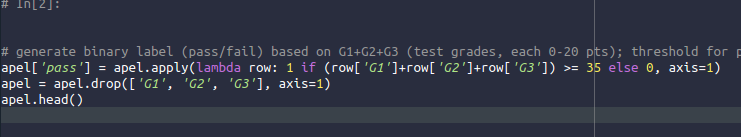
\includegraphics[scale=0.4]{figures/chapter2/chapter1.2.PNG}
		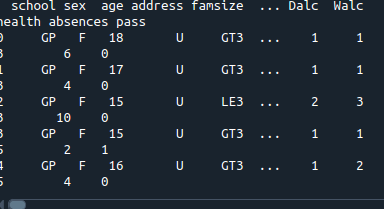
\includegraphics[scale=0.5]{figures/chapter2/hasilchapter1.2.PNG}
		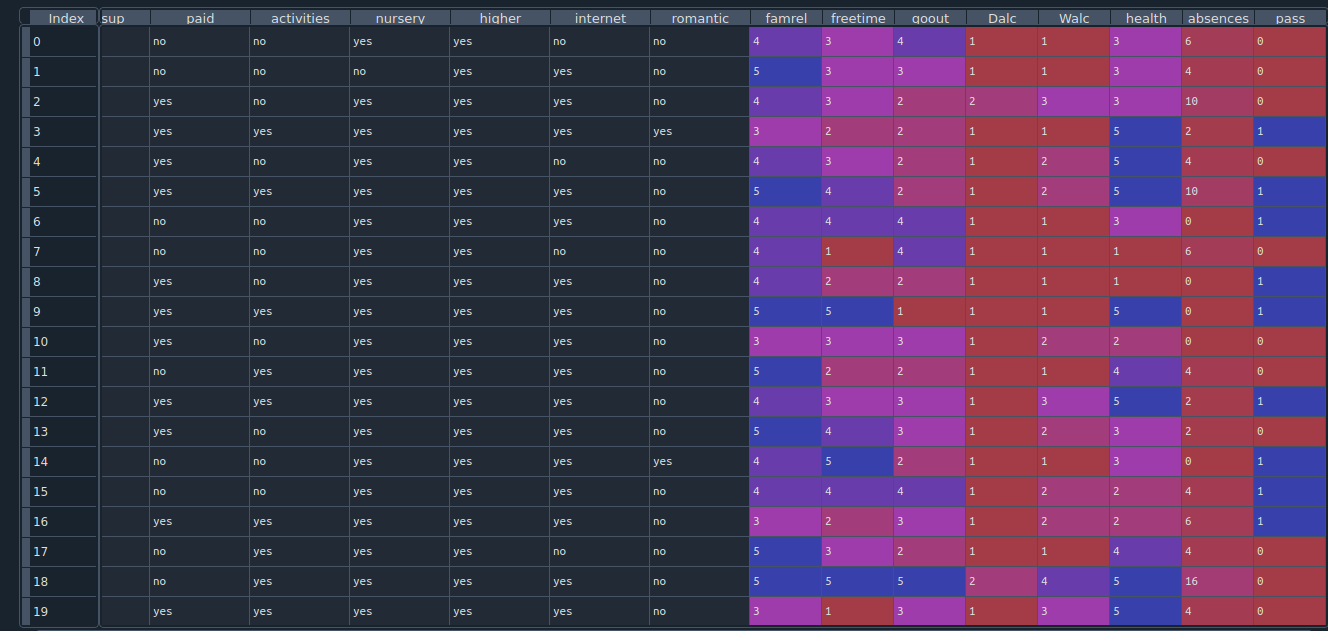
\includegraphics[scale=0.5]{figures/chapter2/hasilchapter1.2.1.PNG}
	\end{figure}
\newpage
\item
\begin{verbatim}
	# use one-hot encoding on categorical columns
	d = pd.get_dummies(d, columns=['sex', 'school', 'address', 
									'famsize', 
									'Pstatus', 'Mjob', 'Fjob', 
	                               'reason', 'guardian', 'schoolsup', 
								   'famsup', 'paid', 'activities',
	                               'nursery', 'higher', 'internet', 
									'romantic'])
	d.head()
\end{verbatim}
\begin{figure}[!htbp]
		\centering
		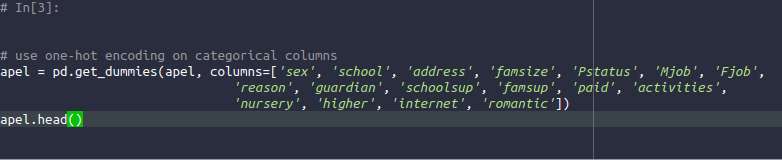
\includegraphics[scale=0.4]{figures/chapter2/chapter1.3.PNG}
		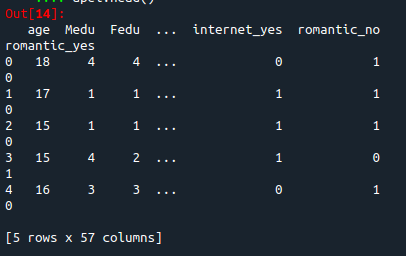
\includegraphics[scale=0.5]{figures/chapter2/hasilchapter1.3.PNG}
	\end{figure}
\newpage
\item
\begin{verbatim}
	# shuffle rows
	d = d.sample(frac=1)
	# split training and testing data
	d_train = d[:500]
	d_test = d[500:]

	d_train_att = d_train.drop(['pass'], axis=1)
	d_train_pass = d_train['pass']

	d_test_att = d_test.drop(['pass'], axis=1)
	d_test_pass = d_test['pass']

	d_att = d.drop(['pass'], axis=1)
	d_pass = d['pass']

	# number of passing students in whole dataset:
	import numpy as np
	print("Passing: %d out of %d (%.2f%%)" % (np.sum(d_pass), len(d_pass), 
	       100*float(np.sum(d_pass)) / len(d_pass)))
\end{verbatim}
\begin{figure}[!htbp]
		\centering
		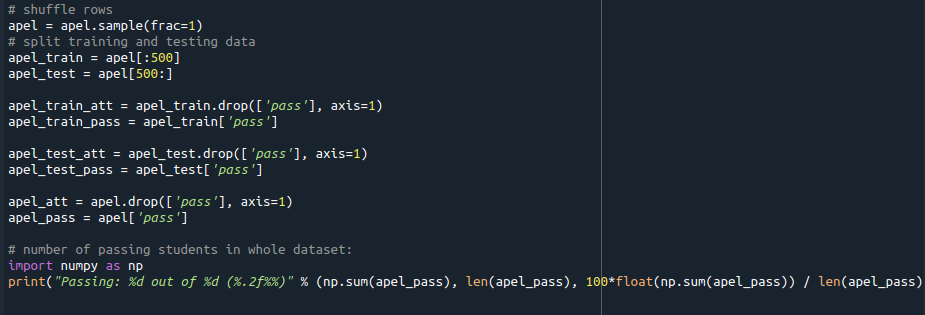
\includegraphics[scale=0.4]{figures/chapter2/chapter1.4.PNG}
		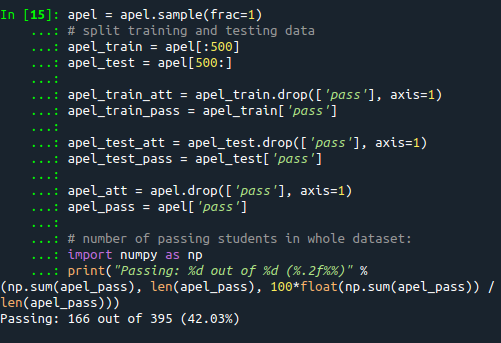
\includegraphics[scale=0.5]{figures/chapter2/hasilchapter1.4.PNG}
	\end{figure}
\newpage
\item 
\begin{verbatim}
	# fit a decision tree
	from sklearn import tree
	t = tree.DecisionTreeClassifier(criterion="entropy", max_depth=5)
	t = t.fit(d_train_att, d_train_pass)
\end{verbatim}
\begin{figure}[!htbp]
		\centering
		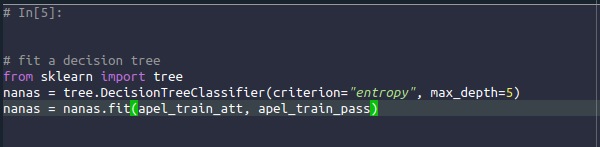
\includegraphics[scale=0.4]{figures/chapter2/chapter1.5.PNG}
		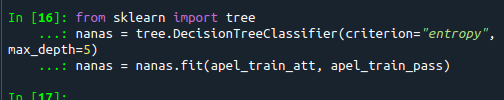
\includegraphics[scale=0.5]{figures/chapter2/hasilchapter1.5.PNG}
	\end{figure}
\newpage
\item
\begin{verbatim}
	# visualize tree
	import graphviz
	dot_data = tree.export_graphviz(t, out_file=None, label="all", 
									impurity=False, proportion=True,
	                                feature_names=list(d_train_att), 
									class_names=["fail", "pass"], 
	                                filled=True, rounded=True)
	graph = graphviz.Source(dot_data)
	graph
\end{verbatim}
\begin{figure}[!htbp]
		\centering
		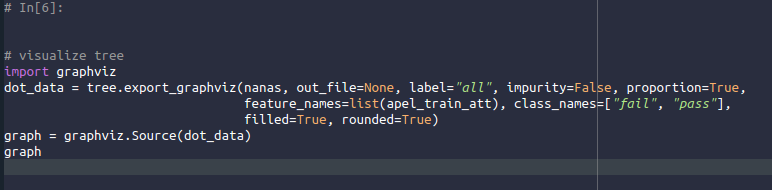
\includegraphics[scale=0.4]{figures/chapter2/chapter1.6.PNG}
		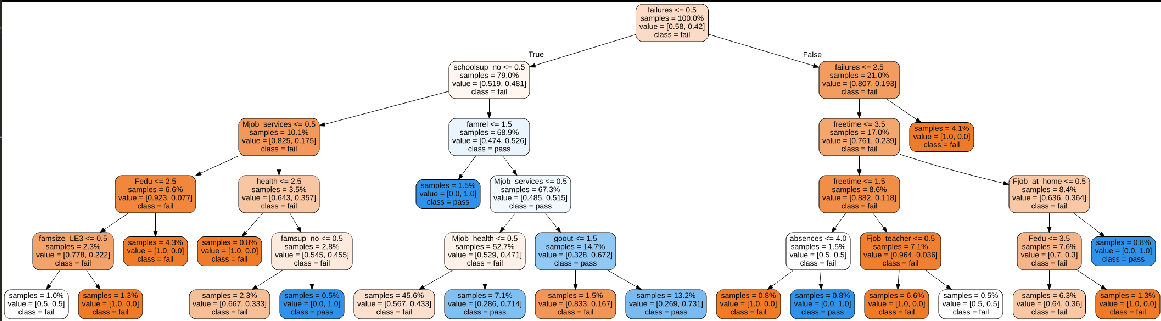
\includegraphics[scale=0.5]{figures/chapter2/hasilchapter1.6.1.PNG}
	\end{figure}
\newpage
\item
\begin{verbatim}
	# save tree
	tree.export_graphviz(t, out_file="student-performance.dot", 
						 label="all", impurity=False, 
						 proportion=True,
	                     feature_names=list(d_train_att), 
	                     class_names=["fail", "pass"], 
	                     filled=True, rounded=True)
\end{verbatim}
\begin{figure}[!htbp]
		\centering
		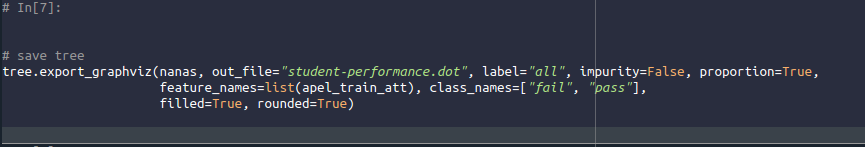
\includegraphics[scale=0.4]{figures/chapter2/chapter1.7.PNG}
		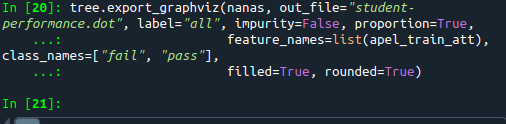
\includegraphics[scale=0.5]{figures/chapter2/hasilchapter1.7.PNG}
		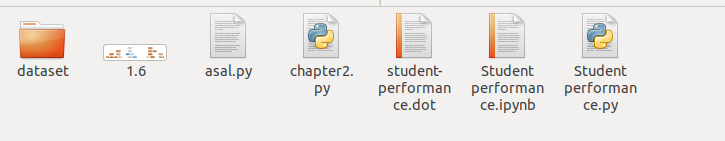
\includegraphics[scale=0.5]{figures/chapter2/hasilchapte1.7.2.PNG}
	\end{figure}
\newpage
\item
\begin{verbatim}
	t.score(d_test_att, d_test_pass)
\end{verbatim}
\begin{figure}[!htbp]
		\centering
		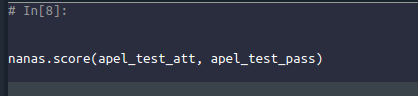
\includegraphics[scale=0.4]{figures/chapter2/chapter1.8.PNG}
		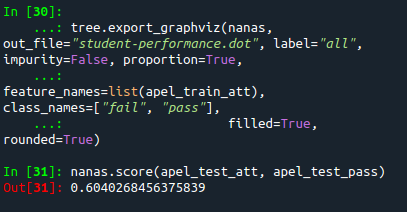
\includegraphics[scale=0.5]{figures/chapter2/hasilchapter1.8.PNG}
	\end{figure}
\newpage
\item
\begin{verbatim}
	from sklearn.model_selection import cross_val_score
	scores = cross_val_score(t, d_att, d_pass, cv=5)
	# show average score and +/- two standard deviations away 
	#(covering 95% of scores)
	print("Accuracy: %0.2f (+/- %0.2f)" % (scores.mean(), scores.std() * 2))
\end{verbatim}
\begin{figure}[!htbp]
		\centering
		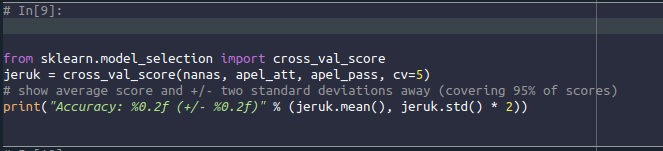
\includegraphics[scale=0.4]{figures/chapter2/chapter1.9.PNG}
		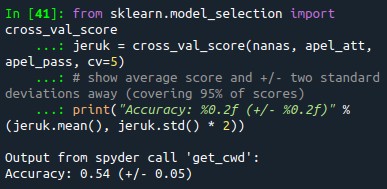
\includegraphics[scale=0.5]{figures/chapter2/hasilchapter1.9.PNG}
	\end{figure}
\newpage
\item 
\begin{verbatim}
	for max_depth in range(1, 20):
	    t = tree.DecisionTreeClassifier(criterion="entropy", 
			max_depth=max_depth)
	    scores = cross_val_score(t, d_att, d_pass, cv=5)
	    print("Max depth: %d, Accuracy: %0.2f (+/- %0.2f)" % 
				(max_depth, scores.mean(), scores.std() * 2)
			 )
\end{verbatim}
\begin{figure}[!htbp]
		\centering
		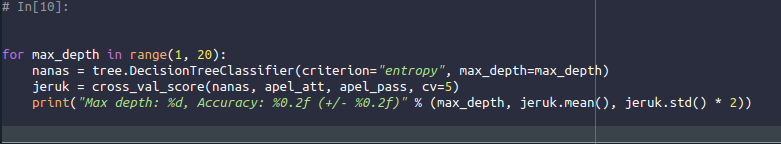
\includegraphics[scale=0.4]{figures/chapter2/chapter1.10.PNG}
		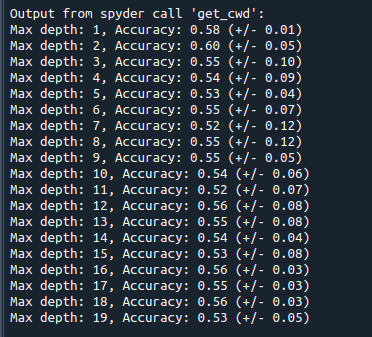
\includegraphics[scale=0.5]{figures/chapter2/hasilchapter1.10.PNG}
	\end{figure}
\newpage
\item
\begin{verbatim}
	depth_acc = np.empty((19,3), float)
	i = 0
	for max_depth in range(1, 20):
	    t = tree.DecisionTreeClassifier(criterion="entropy", 
			max_depth=max_depth)
	    scores = cross_val_score(t, d_att, d_pass, cv=5)
	    depth_acc[i,0] = max_depth
	    depth_acc[i,1] = scores.mean()
	    depth_acc[i,2] = scores.std() * 2
	    i += 1

	depth_acc
\end{verbatim}
\begin{figure}[!htbp]
		\centering
		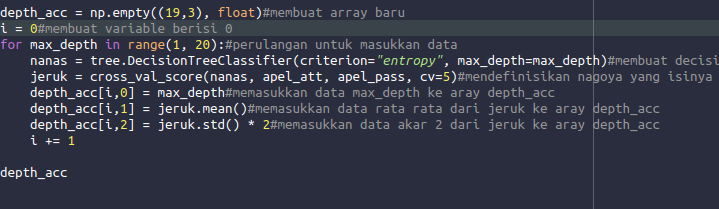
\includegraphics[scale=0.4]{figures/chapter2/chapter1.11.PNG}
		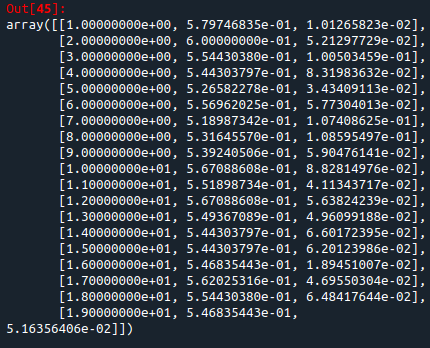
\includegraphics[scale=0.5]{figures/chapter2/hasilchapter1.11.PNG}
	\end{figure}
\newpage
\item 
\begin{verbatim}
	import matplotlib.pyplot as plt
	fig, ax = plt.subplots()
	ax.errorbar(depth_acc[:,0], depth_acc[:,1], yerr=depth_acc[:,2])
	plt.show()
\end{verbatim}
\begin{figure}[!htbp]
		\centering
		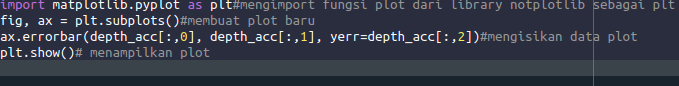
\includegraphics[scale=0.4]{figures/chapter2/chapter1.12.PNG}
		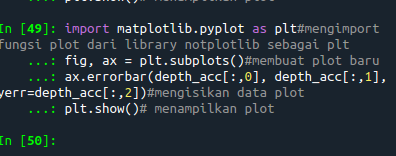
\includegraphics[scale=0.5]{figures/chapter2/hasilchapter1.12.PNG}
	\end{figure}
\newpage

\end{enumerate}


\section{Penanganan Error}
Dari percobaan yang dilakukan di atas, error yang kita dapatkan di dokumentasikan dan di selesaikan(nilai 5 hari kedua):

\begin{enumerate}
	\item
skrinsut error
\begin{figure}[!htbp]
		\centering
		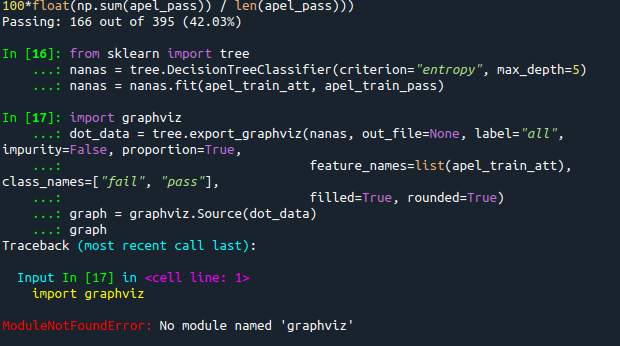
\includegraphics[scale=0.4]{figures/chapter2/instalgravis.png}
		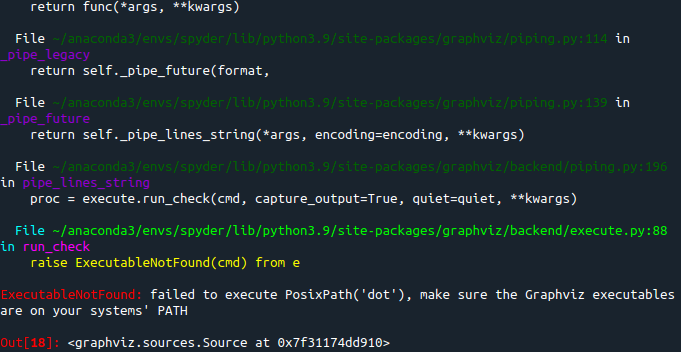
\includegraphics[scale=0.5]{figures/chapter2/setelah instal gravis ttep.png}
	\end{figure}
\newpage
	\item
Tuliskan kode eror dan jenis errornya\\
ModulNotFoundEror: no modul named 'graphviz'\\
ExecutableNotFound: failed to execute posixPath('dot'), make sure the Graphviz executables are in your system PATH\\
Jenis erornya adalah tidak adanya modul didalamnya dan masih kurang ketika di instal modulnya\\
Solusinya dengan melakukan instal modul.
	\item
Solusi pemecahan masalah error tersebut
\begin{figure}[!htbp]
		\centering
		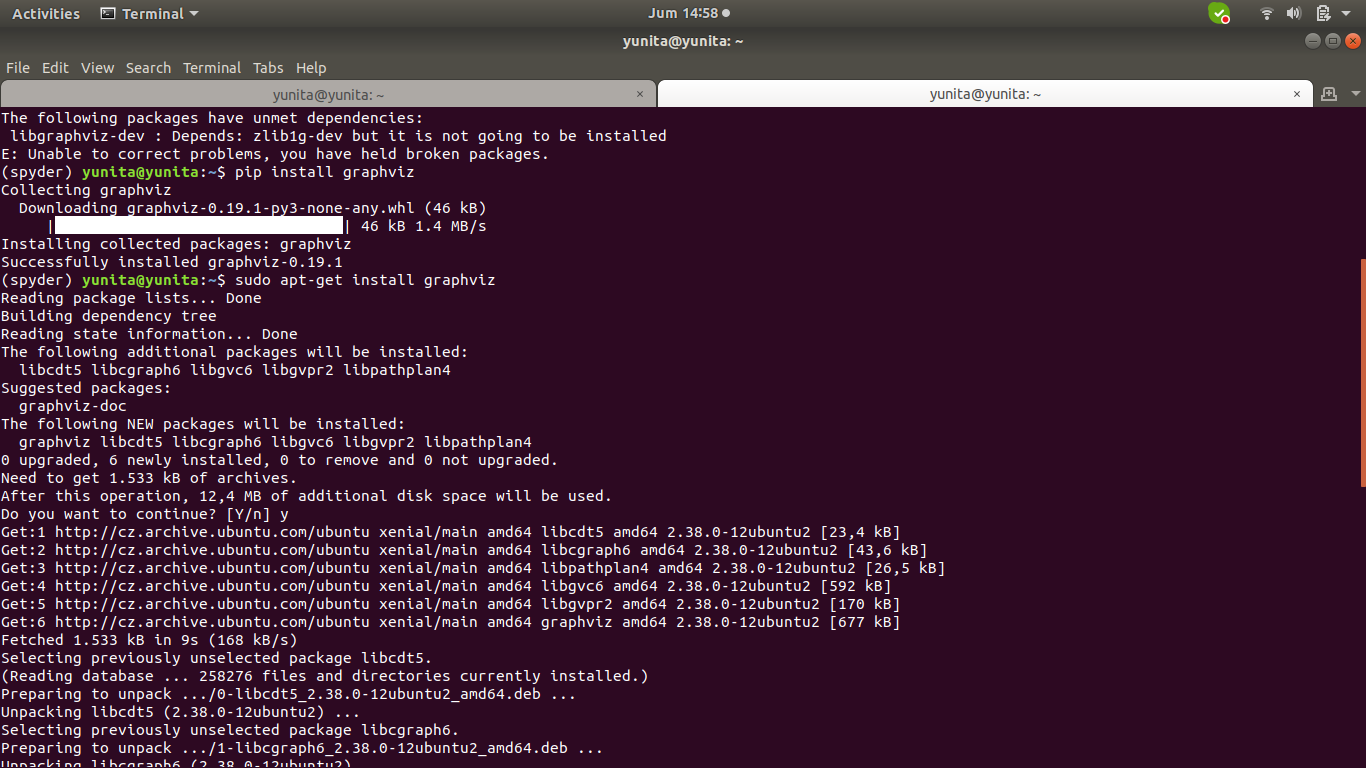
\includegraphics[scale=0.4]{figures/chapter2/ketikaerortidak terdapatmodulgrafis.png}
		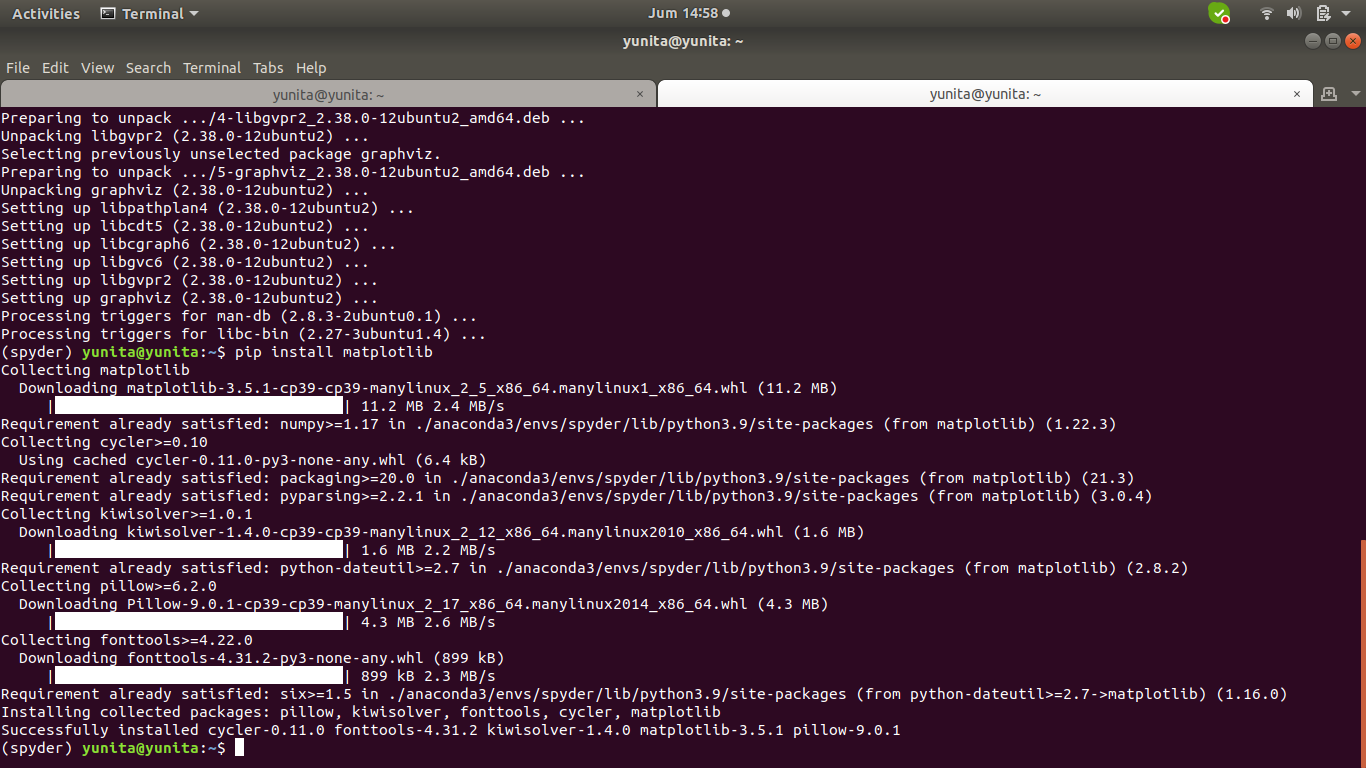
\includegraphics[scale=0.4]{figures/chapter2/erorketikatidakadamodulmatplolib.png}
	\end{figure}

\end{enumerate}

